\chapter{Learning Room Occupancy based on User Routines}

In this chapter, we investigate how a robot can learn occupancy period of different rooms of a office or home based on user's routine. Occupancy represents the belief of the robot about when are rooms occupied or empty. The probabilistic model developed in the previous chapter enables a domestic service robot to learn the user preference for object placement on each locations. We use the same models in this chapter to learn about the occupancy of each rooms

We consider the example of a cleaning robot which needs to decide what time of the day is best suited for cleaning. \cite{Fink2013} did a exhaustive survey about usage, adoption process and long-term effects of domestic cleaning robot in people's homes. One of the biggest barrier for better adoption of robots in household was compatibility with habits and routines. Thus in order for a robot to clean a house or office with minimum intervention, it should have the ability to fully understand its user routines, to make decisions based on the state of each rooms. Thus if the robots can learn the  least occupancy time of the environment it can make decisions on cleaning time which will cause minimum interference for humans. 


In this chapter the robot will learn multiple user's routine in using different rooms of a office and determine the low occupancy time for cleaning.
The robot might use a camera sensor and standard person detection algorithm to detect the human. This generated information are recorded by the robot in its robot memory along with the time and room of the observations. We develop a Bayesian model which can learn from these observations and generate the occupancy periods for each room. In particular, our approach allows a robot (1) to infer the occupancy time of each room (2) to make predictions about future occupancy of each rooms. In our experiments, we demonstrate that robots with our models can learn and predict accurately if a room is occupied.

In the next section we will explain the model used to learn the occupancy periods of each rooms. 

\section{Hierarchical Beta Bernoulli Model}

Hierarchical Beta Bernoulli model explained in Chapter~\ref{chapter: object} is also used to model the occupancy of each room. In Chapter~\ref{chapter: object} the observation were boolean values representing the presence of an object at a particular location. The observations here is also a boolean value representing if the room is occupied. From these boolean observations we need to learn the latent knowledge about the occupancy, and we use the Bernoulli distribution to represent these observations, while the latent occupancy of the room is represented by the Beta distribution. 
Now the model learns the latent knowledge about the occupancy separately for each hour of the day. To enable sharing of knowledge between different times of the day we use the third level of the model, which forms the conjugate prior for the Beta distribution. These ensure the knowledge about latent factor in 1 time period are shared with other time periods. 

\noindent
\begin{figure}[htp]

\begin{minipage}{0.3\textwidth}
\centering

\tikz {
 % Define nodes
  \node[latent]                                 (theta) {$\theta$};
  \node[latent, above=of theta, xshift=-1.2cm]  (alpha) {$\alpha$};
  \node[latent, above=of theta, xshift=1.2cm]   (beta) {$\beta$};
  \node[obs, below=of theta]                    (y)     {$x$}; 
  % Connect the nodes
  \edge {alpha,beta} {theta} ; %
  \edge {theta} {y};
  % plates
  \plate {location} {(y)} {location};
  \plate {time} {(theta)(y)(location)} {time};
}

\end{minipage}%
\begin{minipage}{0.7\textwidth}

\begin{equation*}
	\alpha \sim Beta(2,2) ; \beta \sim Beta(2, 2);
\end{equation*}
\begin{equation*}
	\theta \sim Beta(\alpha, \beta);
\end{equation*}
\begin{equation*}
	x = Bernoulli(\theta)
\end{equation*}
\end{minipage}
\caption[Hierarchical Beta Bernoulli graphical model]{Graphical model representation of Hierarchical Beta Bernoulli model. The boxes are ``plates" representing replicates. The outer plates represents hours of a day, while the inner plate represents if the room has users in that hour.}
\label{bbm2}
\end{figure}



The model can be explained as:

	\boldmath{$\alpha$} and \boldmath{$\beta$} is  prior beta distribution, 
	
	$\theta_i$ is the latent occupancy distribution for period $i$  ,
	
	$x_{ij}$ is the observation in period $i$.


\begin{figure}
    \centering
    \begin{subfigure}[b]{0.21\textwidth}
        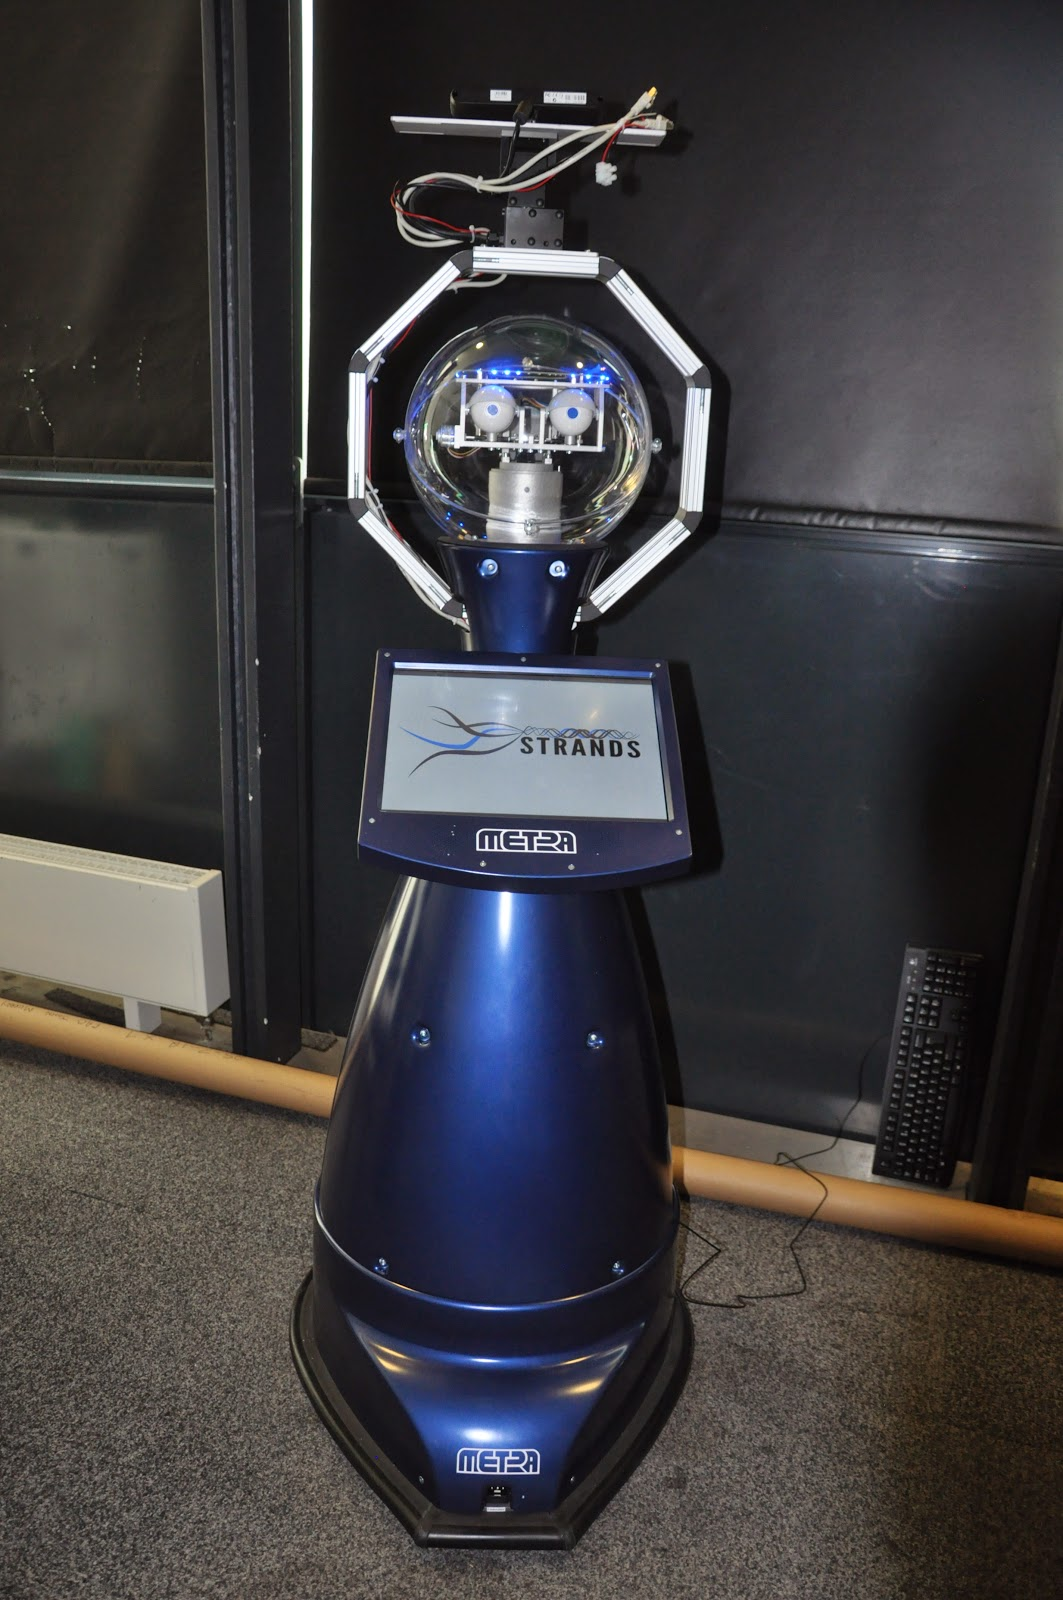
\includegraphics[width=\textwidth]{images/scitos.jpg}
        \caption{}
        \label{fig:scitos-1}
    \end{subfigure}
    ~ %add desired spacing between images, e. g. ~, \quad, \qquad, \hfill etc. 
      %(or a blank line to force the subfigure onto a new line)
    \begin{subfigure}[b]{0.6\textwidth}
        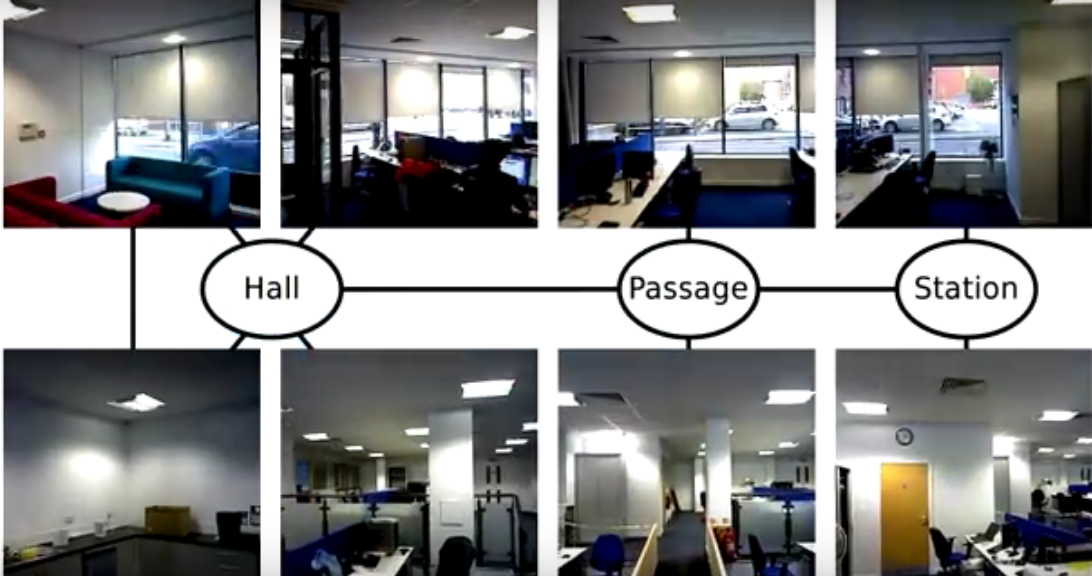
\includegraphics[width=\textwidth]{images/kth-dataset-2.png}
        \caption{}
        \label{fig:robot-view-1}
    \end{subfigure}
    \caption[Brayford dataset collection]{Brayford Dataset collection: SCITOS-G5\footnotemark Robot used for data collection \ref{fig:scitos-1} \protect. Images \footnotemark as seen by the robot at the different rooms in the lab \ref{fig:robot-view-1}}\label{fig:brayford-dataset}
\end{figure}

\footnotetext{\url{ http://www.hanheide.net/2013/06/brand-new-robot.html}}
\footnotetext{\url{https://www.youtube.com/watch?v=aTr9KD4XMGc }}


\section{Experiments}
We conducted our experiments on real data collected by a robot in an office environment. The robot for each room in the office makes observation of its occupancy. The goal of the experiment was to verify that
\begin{itemize}
    \item the robot is able to learn the room occupancy probability.
	\item the resulting model allows for accurate prediction or future occupancy of the room
\end{itemize}

\subsection{Evaluation of Model accuracy}

We evaluated the model accuracy using cross-validation methods on the Brayford dataset. Brayford dataset is extracted from the Witham Wharf RGB-D dataset, both collected as part of the Spatio-Temporal Representations and Activities for Cognitive Control in Long-Term Scenarios (STRANDS) project. 
Witham Wharf RGB-D dataset is used for testing RGB-D localization in changing environments. The dataset consist of RGB-D images collected over eight locations in an open-plan office. The Brayford dataset was extracted from the above dataset by manually annotating the presence of human in the room at the moment. Figure~\ref{fig:brayford-dataset} shows the data collection method. Data was collected using the SCITOS-G5 robot. 



\begin{figure}[htp]
\centering
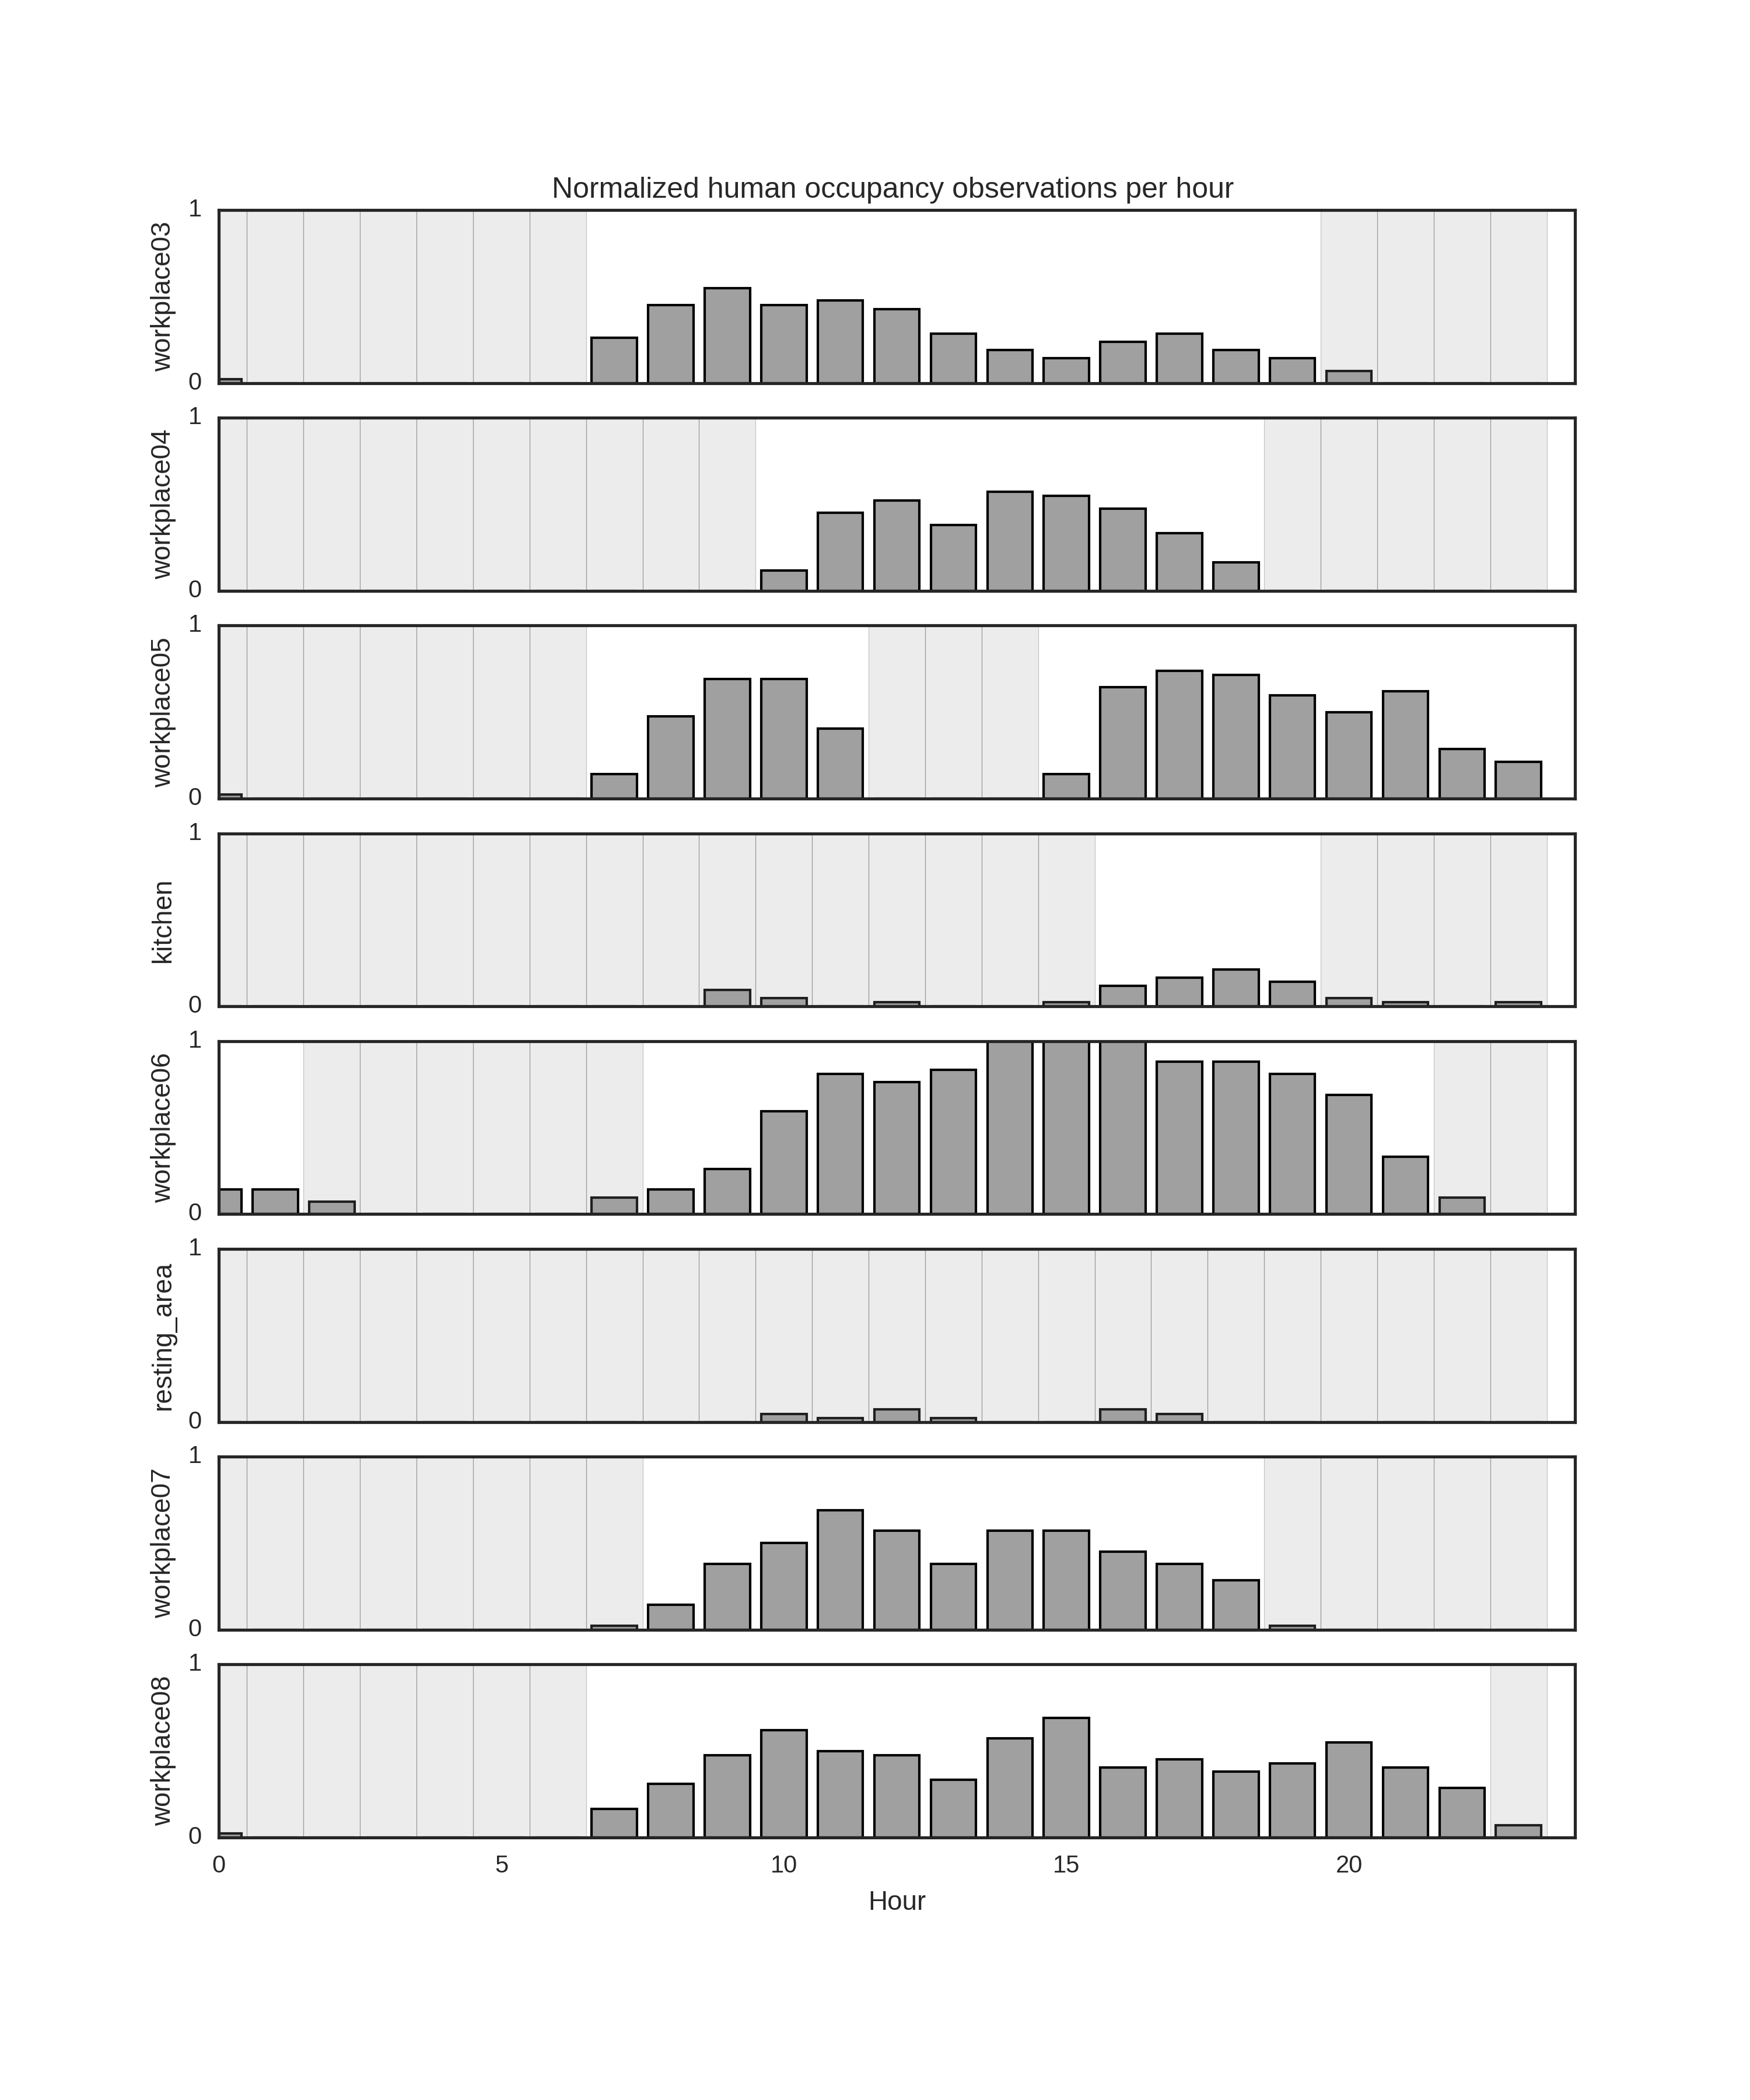
\includegraphics[width=\textwidth]{images/occupancy_hist_withresults.png}
\caption[Brayford Dataset ]{Brayford Dataset: normalized human occupancy per hour per room. The shaded regions are the learned cleaning time period for each room.}
\label{fig:brayford_visualization}
\end{figure}

\FloatBarrier



The dataset is divided in 2 parts the training set and testing set. The training set consist of 7 days of observations, where the robot visits predefined eight locations of the office at a regular interval of 10 minutes each. The testing set consist of another week of observation. Figure~\ref{fig:brayford_visualization} is the bar plot of the observations made by the robot. 



The training dataset was used to learn the parameters of the model while the testing dataset was used to predict and validate the learned models. 
The accuracy results of the 8 rooms is plotted in Figure~\ref{fig:brayford_evaluation} . The model predicts with above \textbf{80\%} accuracy for 3 rooms kitchen, resting area and workplace04 . While accuracy of predictions for other rooms are in the range of 60\% to 80\% .

\begin{figure}[htp]
\centering
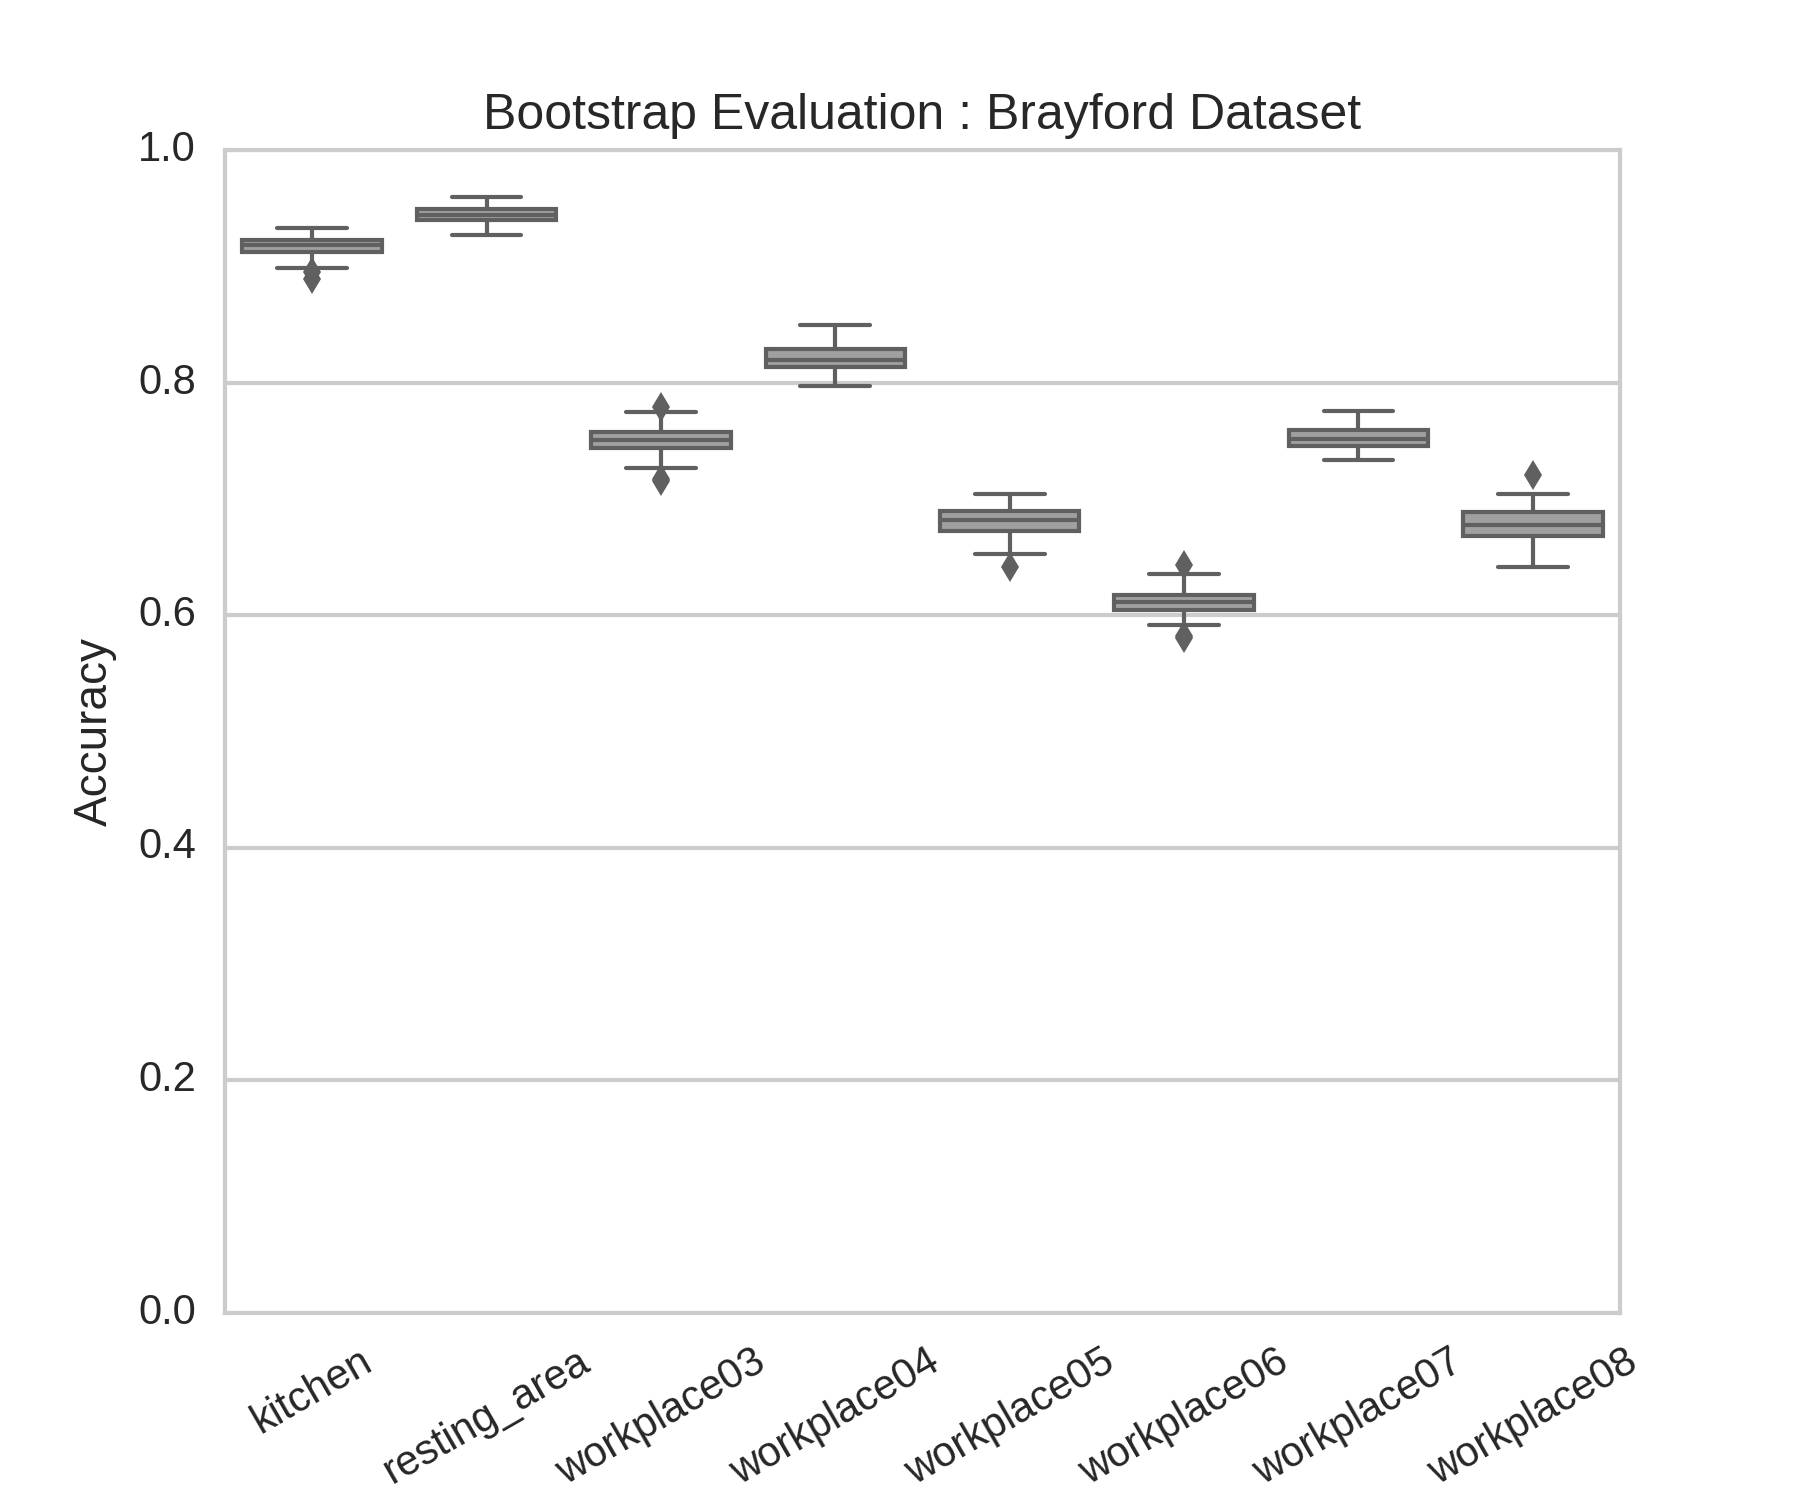
\includegraphics[width=0.7\textwidth]{images/Brayford_dataset_results_evaluation.png}
\caption[Brayford Dataset Evaluation]{Brayford dataset evaluation: Accuracy of the model for different rooms in the office}
\label{fig:brayford_evaluation}
\end{figure}



Based on the learned occupancy parameter for each room, the robot can now determine which are the period of low occupancy and select these time periods for doing its cleaning task. The shaded region in the Figure~\ref{fig:brayford_visualization} are the learned time periods in which the robot can perform cleaning task.
\FloatBarrier

\section{Discussions}

In this chapter, we presented a probabilistic framework for learning the occupancy periods of each rooms. The robot continuously records in its robot memory when and where it saw the users. Now based on the data collected the robot now does an analysis gain knowledge about the occupancy of each room. 

We have used the identical model as discussed in chapter ~\ref{chapter: object} for learning the occupancy parameter. This demonstrates the flexibility of the probabilistic programming in which we can reuse the models to new problems.
From the experiments conducted on real world datasets collected by mobile robots in an open office we can conclude that the model is able to learn accurately the latent occupancy time periods. 